\documentclass[a4paper,12pt]{extarticle}
\usepackage{geometry}
\usepackage[T1]{fontenc}
\usepackage[utf8]{inputenc}
\usepackage[english,russian]{babel}
\usepackage{amsmath}
\usepackage{amsthm}
\usepackage{amssymb}
\usepackage{fancyhdr}
\usepackage{setspace}
\usepackage{graphicx}
\usepackage{colortbl}
\usepackage{tikz}
\usepackage{pgf}
\usepackage{subcaption}
\usepackage{listings}
\usepackage{indentfirst}
\usepackage[colorlinks,citecolor=blue,linkcolor=blue,bookmarks=false,hypertexnames=true, urlcolor=blue]{hyperref} 
\usepackage{indentfirst}
\usepackage{mathtools}
\usepackage{booktabs}
\usepackage[flushleft]{threeparttable}
\usepackage{tablefootnote}
\usepackage{pdfpages}

\usepackage{chngcntr} % нумерация графиков и таблиц по секциям
\counterwithin{table}{section}
\counterwithin{figure}{section}

\graphicspath{{graphics/}}%путь к рисункам

\usepackage{pdflscape}

\makeatletter
\renewcommand{\@biblabel}[1]{#1.} % Заменяем библиографию с квадратных скобок на точку:
\makeatother

\geometry{left=3cm}% левое поле ГОСТ!!!
\geometry{right=1.5cm}% правое поле
\geometry{top=2cm}% верхнее поле ГОСТ!!!
\geometry{bottom=2cm}% нижнее поле ГОСТ!!!
\renewcommand{\baselinestretch}{1.5} % междустрочный интервал


\newcommand{\bibref}[2]{\hyperlink{#1}{#2}} % biblabel, authors, year
\addto\captionsrussian{\def\refname{Список литературы}} 

\renewcommand{\theenumi}{\arabic{enumi}}% Меняем везде перечисления на цифра.цифра
\renewcommand{\labelenumi}{\arabic{enumi}}% Меняем везде перечисления на цифра.цифра
\renewcommand{\theenumii}{.\arabic{enumii}}% Меняем везде перечисления на цифра.цифра
\renewcommand{\labelenumii}{\arabic{enumi}.\arabic{enumii}.}% Меняем везде перечисления на цифра.цифра
\renewcommand{\theenumiii}{.\arabic{enumiii}}% Меняем везде перечисления на цифра.цифра
\renewcommand{\labelenumiii}{\arabic{enumi}.\arabic{enumii}.\arabic{enumiii}.}% Меняем везде перечисления на цифра.цифра

\usepackage{Style/code}

\begin{document}
\renewcommand{\thelstlisting}{\thesection.\arabic{lstlisting}}

% \begin{titlepage}
    \newpage
    
    {\setstretch{1.0}
    \begin{center}
    ПРАВИТЕЛЬСТВО РОССИЙСКОЙ ФЕДЕРАЦИИ\\
    ФГАОУ ВО НАЦИОНАЛЬНЫЙ ИССЛЕДОВАТЕЛЬСКИЙ УНИВЕРСИТЕТ\\
    «ВЫСШАЯ ШКОЛА ЭКОНОМИКИ»
    \\
    \bigskip
    Факультет компьютерных наук\\
    Образовательная программа «Прикладная математика и информатика»
    \end{center}
    }
    
    \vspace{2em}
    %УДК 51-7 % УДК нужно указывать только для исследовательсвого проекта - удалите эту строку для программного проекта
    \vspace{4em}
    
    \begin{center}
    %Выберите какой у вас проект
    % {\bf Отчет об исследовательском проекте на тему:}\\
    %{\bf Отчет о командном исследовательском проекте на тему:}\\
    {\bf Отчет о программном проекте на тему:}\\
    %{\bf Отчет о командном программном проекте на тему:}\\
    {\bf Многофункциональный поисковой движок для индексирования
    документов}\\
    % строчка ниже нужна только при сдача плана КР, при финальной сдаче закомментируйте ее
    %(промежуточный, этап 1)
    \end{center}
    
    \vspace{2em}
    
    {\bf Выполнил студент:\vspace{2mm}}
    
    {\setstretch{1.1}
    \begin{tabular}{l@{\hskip 1.5cm}l}
    группы \#БПМИ238, 2 курса 
    \\ Поляков Иван Андреевич & 01.04.2025 \\ & \hspace{2mm} \textit{\footnotesize (дата)} \\
    \end{tabular}}
    
    % Обычно у вас есть один научный руководитель, и это человек, с которым вы работаете над проектом. Иногда по формальным причинам у вас будет руководитель (штатный сотрудник Вышки) и соруководитель (тот, с кем вы работаете), — об этом вам сообщит учебный офис (в случае с ВКР) или ЦППРиП (в случае с курсовым проектом). Также, если кто-то дополнительно вам помогал, то его можно указать как консультанта. 
    
    \vspace{1em}
    {\bf Принял руководитель проекта: \vspace{2mm}}
    
    {\setstretch{1.1}
    \begin{tabular}{l}
    Садуллаев Музаффар Тимурович\\
    Приглашенный преподаватель, \\
    Департамент больших данных и информационного поиска\\
    Факультет компьютерных наук НИУ ВШЭ 
    \end{tabular}}
    
    
    \vspace{\fill}
    
    \begin{center}
    Москва 2025
    \end{center}
    
    \end{titlepage}% это титульный лист
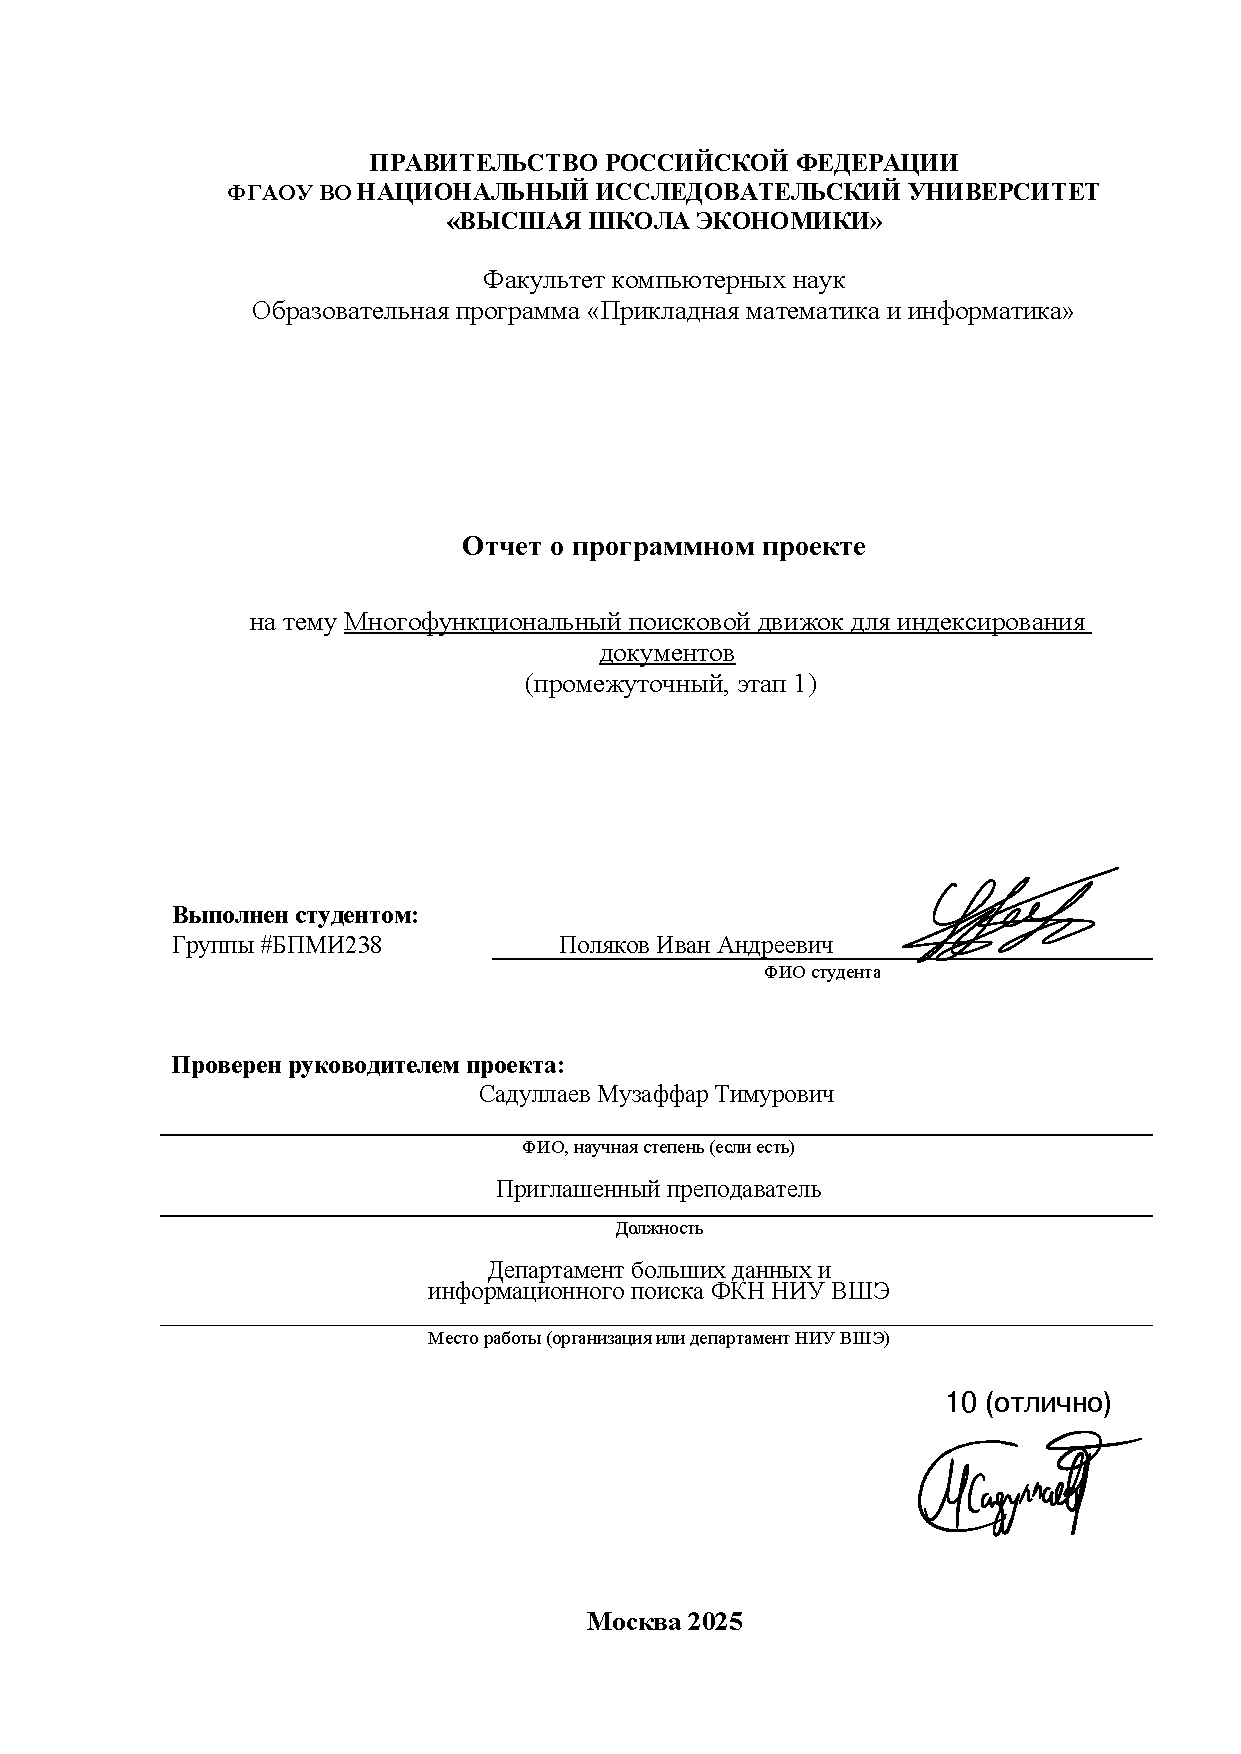
\includepdf{new_title.pdf}

\newpage
\setcounter{page}{2}
{
	\hypersetup{linkcolor=black}
	\tableofcontents
}
\newpage
% \section{Основные термины и определения}
% \begin{enumerate}
%     \item \textbf{Морфема} - наименьшая единица языка, имеющая некоторое значение. (Корни и аффиксы: приставки, суффиксы, окончания и т.п.) \cite{wiki_morph}.
%     \item \textbf{Семантика} - раздел лингвистики, изучающий смысловое значение единиц языка \cite{wiki_semantika}.
% \end{enumerate}

\newpage 
\section{Введение}
\subsection{Цель}
Цель работы заключается в разработке легковесного и многофункционального поискового движка для работы с различными данными. 

\subsection{Задачи}
\begin{itemize}
  \item{Исследовательская часть}
    \begin{itemize}
        \item {Изучить существующие поисковые движки, изучить их устройство и используемые технологии}
        \item {Изучить процесс токенизации, рассмотреть существующие библиотеки}
        %...
    \end{itemize}
  \item{Программная часть}
      \begin{itemize}
        \item{Разработать алгоритм токенизации, позволяющий за короткий временной промежуток обрабатывать большие объемы документов}
        \item {Разработать алгоритм для преобработки текста, который будет включать в себя такие части как токенизация, нормализация и стемминг}
        \item {Построить инвертированный индекс для последующего поиска}
        \item {Реализовать хранение индекса  в базе данных}
        \item {Разработать алгоритм ранжирования результатов поиска}
        \item{Реализовать графическую оболочку для вывода результатов поиска}
    \end{itemize}
\end{itemize}

\subsection{Актуальность работы}
На рынке представлено множество различных поисковых движков, однако большая часть отличается обширной кодовой базой и 
большими системными требованиями. Среди крупных игроков рынка можно выделить Google, Yandex, Baidu, Yahoo, Bing. 
Все эти компании разработали собственные поисковые движки, которые являются готовыми продуктами и ими пользуются 
ежедневно миллиарды человек. Однако их главная  проблема все еще в том, что их работа требует огромных производительных 
мощностей. Мой движок должен стать компромиссным решением, которое будет сочетать в себе многофункциональный поиск 
по нескольким типам файлов и обладать достаточной легковестностью. Таким образом можно считать, 
что актуальность работы продемонстрирована.

\subsection{План работы}
\begin{itemize}
    \item{Проанализировать существующие поисковые движки, изучить их \\
    устройство и используемые технологии}
    \item {Изучить процесс токенизации, рассмотреть существующие библиотеки}
    \item {Имплементировать алгоритм токенизации, позволяющий за короткий временной промежуток обрабатывать большие объемы документов }
    \item {Имплементировать веб-краулер для рекурсивного обхода веб-страниц и извлечения из них различных данных для индексирования}
    \item {Реализовать хранение индекса в базе данных, проработать ее эффективное взаимодействие с остальной программой}
    \item {Имплементировать поиск данных в индексе на основе поискового запроса пользователя }
    \item {Реализовать алгоритм ранжирования полученных результатов поиска}
    \item {Разработать графическую оболочку для просмотров результатов поиска}
  \end{itemize}
\newpage
\section{Существующие поисковые движки}
%Включает в себя обзор источников и раскрытие темы
Если мы говорим про крупнейшие поисковые движки, то в силу закрытого исходного кода, то мы не можем знать, 
какие именно алгоритмы токенизации и ранжирования они используют, однако существует масса решение с открытым 
исходным кодом. Среди самых используемых можно выделить Elasticsearch и Solr. Рассмотрим каждый из них и 
выделим, какие их части можно интегрировать в мой движок.

\subsection{Elasticsearch}
В первую очередь это поисковой движок для поиска по документам. Этот движок использует построение инвертированного 
индекса - индекса, который сопоставляет токенам соответствующие документы, в которых они встретились. Для этого используется 
библиотека Apache Lucene. Также в Elasticsearch может использоваться распределенный индекс - он хранится на нескольких 
серверах, что позволяет организовать горизонтальное масштабирование. Для эффективного поиска этот движок использует 
специальные метрики узлов - базы данных для хранения индекса - позволяющие распределять нагрузку по нескольким серверам. 

\subsection{Solr}
Начиная с 2010 года Solr и Lucene были объединены. Solr это Apache Lucene с дополнительным функционалом - поиском. 
Он использует всю ту же библиотеку Apache Lucene для построения инвертированного индекса, но добавляет алгоритм поиска 
и ранжирования результатов. 

\subsection{Вывод}
Из анализа существующих решений с открытым исходным кодом можно сделать вывод, что в моем поисковом движке следует 
также использовать инвертированных индекс, так как он позволяет осуществлять полнотекстовый поиск и сразу по токенам 
получать id релевантных документов. Это замедляет процесс индексирования, но кратно уменьшает время поиска.

Что касается взаимодействия с базой данных, то в связи с тем, что мой движок будет работать с одной физической базой данных, 
то я не буду разрабатывать алгоритмы, схожие с решениями Elasticsearch, однако безусловно стоит детально проработать
эффективное распределение нагрузки при большом количестве запросов.
\enlargethispage{\baselineskip}

% Пример ссылки на Рисунок \ref{fig:choosen_words_graph} и на Таблицу \ref{tab:table1} и на Листинг \ref{lst:listing1}.

% \subsection{Пример вставки и оформления рисунка}
% Текст

% \begin{figure}[h!]
% 	\centering
% 	% \includegraphics[scale=0.5]{images/select_sentences/choosen_words.png}
% 	\caption{График распределения сложности выбранных слов}
% 	\label{fig:choosen_words_graph}
% \end{figure}

% \subsection{Пример вставки и оформления кода}
% Пример того как ссылаться на Листинг \ref{lst:listing1}.

% \begin{lstlisting}[caption=Использование schedule в коде, label=lst:listing1]
% def sched_save():
%     schedule.every().hour.do(log_saver)
%     while True:
%         schedule.run_pending()
%         time.sleep(1)
% \end{lstlisting}

% \subsection{Пример вставки и оформления таблицы}
% Пример того как ссылаться на Таблицу \ref{tab:table1} по тексту.

% \begin{table}[h!]
%   \begin{center}
%     \caption{Your first table.}
%     \label{tab:table1}
%     \begin{tabular}{l|c|r} % <-- Alignments: 1st column left, 2nd middle and 3rd right, with vertical lines in between
%       \textbf{Value 1} & \textbf{Value 2} & \textbf{Value 3}\\
%       $\alpha$ & $\beta$ & $\gamma$ \\
%       \hline
%       1 & 1110.1 & a\\
%       2 & 10.1 & b\\
%       3 & 23.113231 & c\\
%     \end{tabular}
%   \end{center}
% \end{table}
\newpage
\section{Токенизация}
Сама по себе Токенизация это процесс разбиение текста на токены. В зависимости от задачи это можно делать разными 
способами, например, в качестве разделителей использовать только пробелы, или же пробелы и запятые, или же 
токенизировать текст по слогам. В моем проекте необходимо будет не только разбивать тексты различных документов на 
токены, но еще и производить с ними какие-то манипуляции для эффективного индексирования. 

\subsection{Нормализация}
Самый первых шаг это нормализация. В нее входит приведение всех символов к нижнему регистру и преобразование некоторых 
специфических букв различных языков к своим латинским аналогам: å --> a. Далее необходимо производить удаление так 
называемых стоп слов-слов, которые очень часто встречаются в языке, но не несут в себе какой-то смысл, в русском это 
местоимения, предлоги, частицы, междометия и прочее. Они будут встречаться в каждом документе и не будут при этом 
отличать его от других при поиске. После удаления стоп-слов следует провести либо стемминг, либо лемматизацию для 
уменьшения потенциального количества токенов и более качественно поиска. Разберем этот момент подробнее. 

\subsection{Стемминг}
Стемминг это обрезка слова для поиска его основы - она не всегда совпадает с 
морфологическим корнем. Основа - неизменяемая часть слова, которая выражает его. В некоторых реализациях не требуется явного 
использования алгоритмов машинного обучения, 
предполагается возможность обойтись раннее изученными алгоритмами, которые могут решить эту задачу.
Также рассмотрим варианты реализации на русском и английском языках

\subsection{Лемматизация}
Что такое Лемматизация? Это процесс приведения слова к лемме - его нормальной форме. Если говорить проще - то 
это начальная, словарная форма слова. То есть мы не всегда обрезаем слово, а например меняем его окончание/суффикс. 
Безусловно, лемматизация дает более точный по смыслу результат, но ее недостатки заключаются в том, что она требует 
намного больше ресурсов и ее использование зачастую предполагает ML. 

\subsection{Анализ готовых решений}
Существуют библиотеки для различной работы с текстом, его токенизацией, нормализацией и стеммингом. Можно выделить такие решения, как NLTK и SpaCy. 

\subsubsection{NLTK}
NLTK - Natural Language toolkit, это Python библиотека для обработки естественного языка. Она продоставляет широкую 
функциональность, начиная от базовой токенизацией и заканчивая готовыми списками стоп слов на разных языках. 
Предполагается изучение некоторых алгоритмов, которые используются в этой библиотеке и их реализация на Golang. 

\subsubsection{SpaCy}
SpaCy. Эта библиотека Python является аналогом NLTK, однако она быстрее справляется с некоторыми задачами в силу того, что написана на CPython. В процессе реализации алгоритмов стемминга также предполагается изучить их реализацию в этой библиотеке. 


\newpage
\section{Индексирование}
После стемминга или лемматизации наш документ превращается в набор токенов, каждый из которых был 
нормализован и сокращен с помощью специальных алгоритмов. Построение инвертированного индекса заключается 
в сопоставлении токену документов, в которых встретился этот токен. Для эффективной выдачи результатов 
необходимо также ввести метрики, по которой мы будем оценивать, какой документ является более релевантным 
по одному конкретному токену - такой метрикой может быть либо стандартный TF-TDF или же BM25. 
% \newpage
% \section{Заключение}

Здесь кратко то что было сделано. Нужно рассказать какие поставленные задачи были решены и достигнута ли цель. Здесь же указываются ссылки на разработанный проект, и др.

\subsection{Результаты}
По итогам работы ...

Во время написания работы автором были решены следующие задачи:
\begin{itemize}
    \item Пункт 1
    \item Пункт 2
    \item Пункт 3
\end{itemize}

В процессе разработки приобретены и улучшены навыки навыки:
\begin{itemize}
    \item Пункт 1
    \item Пункт 2
    \item Пункт 3
\end{itemize}

\subsection{Развитие работы}

Здесь показываем как можно развивать работу в дальнейшем, какие улучшения можно сделать и т.п.

% \newpage
% \begin{thebibliography}{0}
    
%     \bibitem{wiki_semantika}\hypertarget{wiki_semantika}{}
%     % \href{https://cyberleninka.ru/article/n/sintez-matritsy-dvumernogo-izobrazheniya-so-sverhrazresheniem}{Блажевич С. В., Селютина Е. С. Синтез матрицы двумерного изображения со сверхразрешением // Прикладная математика & Физика. 2012. №23 (142). URL: https://cyberleninka.ru/article/n/sintez-matritsy-dvumernogo-izobrazheniya-so-sverhrazresheniem (дата обращения: 23.11.2024).}
    
%     \bibitem{wiki_morph}\hypertarget{wiki_morph}{}
%     \href{https://ru.wikipedia.org/wiki/%D0%9C%D0%BE%D1%80%D1%84%D0%B5%D0%BC%D0%B0}{Бунин, О. А. TCP против UDP или будущее сетевых протоколов / О. А. Бунин. — Текст : электронный // Хабр : [сайт]. — URL: https://habr.com/ru/companies/oleg-bunin/articles/461829/ (дата обращения: 30.01.2024).}

%     \bibitem{matplolib}\hypertarget{matplotlib}{}
    
%     \href{https://matplotlib.org/stable/index.html}{Matplotlib 3.8.2 documentation. — Текст : электронный // Matplotlib : [сайт]. — URL: https://matplotlib.org/stable/index.html (дата обращения: 28.01.2024).}
    
    
% \end{thebibliography}
\end{document}
